\documentclass[11pt]{article}
%\usepackage{ngerman}
\usepackage[english]{babel}
\usepackage{amsmath,amssymb,amstext}
\usepackage{graphicx}
\usepackage{parskip}
\usepackage{float}
\usepackage{tabularx}
\usepackage{amsmath}
\usepackage{esint}
%\usepackage{subtextbf}
\usepackage{pdfpages}
\usepackage{url}
%\usepackage{cite}
\usepackage{array}
\usepackage{multirow}
\usepackage{hyperref}
\usepackage{biblatex}
\usepackage{todonotes}


 
\bibliography{Documentation/references/references}
\bibliographystyle{plain}
\setlength{\textwidth}{15 true cm}
\setlength{\textheight}{22 true cm}
\oddsidemargin  0.5 cm
\evensidemargin 0.5 cm
\topmargin      0 cm

\renewcommand{\textfraction}{.2}
\renewcommand{\floatpagefraction}{.8}

\begin{document}
%\frontmatter
\pagenumbering{roman}

% Include titlepage
\begin{titlepage}	
	{\sffamily		
		\begin{center}			
			\includegraphics[width=30mm]{images/TU_Graz_Logo.png}
			
			\vfill\vfill\vfill
			\vfill\vfill\vfill
			
			{Simon Prato}
			% Author with existing titles
			
			\vfill\vfill\vfill
			
			{\LARGE\bfseries{Numerical Investigation of TEM Cells and Antenna Coupling}}
			% Title of the thesis			
			
			\vfill\vfill\vfill
			\vfill\vfill\vfill			
			
			{\bfseries\large{Master Thesis}}
			
			{Studies: {Electrical Engineering}}
						
			\vfill\vfill\vfill			
			
			submitted to
			
			\vfill
			
			{\bfseries\large{Technical University of Graz}}			
			
			\vfill\vfill\vfill			
			
			Supervisor
			
			{Dr. Thomas Bauernfeind}
			
			\vfill
			
			\vfill
			
			\includegraphics[width=30mm]{Documentation/images/igte_logo.png}
			
			%% OPTIONAL: second supervisor/name of the faculty, etc.
					
			\vfill\vfill\vfill
					
			{Graz}, {August}~{2024}
			
		\end{center}
	}%% end sffamily
\end{titlepage}

\newpage

% Kurzfassung
\iftrue
\cleardoublepage
\setcounter{page}{2}
\vspace*{2.2 cm}
{\Large
\noindent
{\bf Abstract}} \\
\vspace*{0.3 cm}

\noindent

% Abstract
\cleardoublepage
\fi

\selectlanguage{english}
% Inhaltsverzeichnis
	\tableofcontents  

% Tabellenverzeichnis
% optional
\newpage
	\listoffigures 

% Abbildungsverzeichnis
% optinal
\newpage
	\listoftables
	
\cleardoublepage

%\mainmatter
\pagestyle{headings}
\pagenumbering{arabic}

\section{Introduction}

\section{Theoretical Basics}
\subsection{Dipoles}
\subsubsection{Electric Dipoles}

Modeling the electromagnetic radiation of antennas proves to be a challenging task. Using magnetic and electric dipoles is a way to do this, which is especially well applicable for electrically small antennas, which are used in this document. Electrically small antennas have dimensions which are less than one tenth of the wavelength ($<<\frac{\lambda}{10}$)\cite{Balanis_1997}. By calculating the respective dipole moments, the coupling of the antennas to the TEM cells is numerically estimated. Therefore, this section aims to provide a short introduction to the theory behind this concept.

An electric dipole is often described as two tiny charged metal spheres, which are connected with a linear and thin wire\cite{Griffiths_2024} or simply as an T-antenna containing charged capacitor-plates at the end of the wire \cite{Balanis_1997}. The distance $d$ between those charges is very short compared to the wavelength ($d << \lambda$), therefore the dipole can be approximated as ideal\cite{Griffiths_2024}. The electric dipole moment $\mathbf{p}$ is defined by \autoref{eqn:elec_dipole_mom}\cite{Balanis_1997}\cite{Jackson}. %% Erklärung hier. Besser die Bücher zu referenzieren, als selbst etwas zu erfinden.

\begin{equation}
    \mathbf{p} = \int\mathbf{x'} \rho (\mathbf{x'})\mathrm{d}^3x'
    \label{eqn:elec_dipole_mom}
\end{equation}

\autoref{fig:electric_dipole} demonstrates a simple example of a center-fed dipole with a narrow gap as a feedpoint, for which the electric dipole can be used to calculate its radiation\cite{Griffiths_2024}\cite{Jackson}. A current $I_0$ is injected at the feedpoint, which linearly drops to zero along the antenna arms, as described by \autoref{eqn:current_dipole}\cite{Jackson}.

\begin{equation}
    I(z)= I_0\left( 1-\frac{2|z|}{d} \right)
    \label{eqn:current_dipole}
\end{equation}

%Hier das Ergebnis der Integration anschreiben. Die integration selbst auch anschreiben- 

\begin{figure}[h]
    \centering
    \includegraphics[width=0.5\linewidth]{Documentation//images/electric_dipole_drawing.png}
    \caption{Electric dipole}
    \label{fig:electric_dipole}
\end{figure}

The charge per unit length $\rho'$, approximated due to the thin wire, is then derived by the continuity equation in frequency domain by \autoref{eqn:charge_distribution_dipole}. It is constantly distributed along each antenna arm\cite{Griffiths_2024}\cite{Jackson}.

\begin{equation}
    \rho' = \pm\frac{\mathrm{d}}{\mathrm{d}z}\frac{\mathrm{i}I(z)}{\omega} = \pm\frac{2\mathrm{i}I_0}{\omega d}
    \label{eqn:charge_distribution_dipole}
\end{equation}

Using \autoref{eqn:elec_dipole_mom} leads to the resulting electric dipole moment in \autoref{eqn:dipole_mom_example} of this structure. It is parallel to the antenna's arms and points in z-direction\cite{Griffiths_2024}\cite{Jackson}. 

\begin{equation}
    \mathbf{p}=\int_{-\frac{d}{2}}^{\frac{d}{2}}z\rho'(z)\mathrm{d}z\cdot\mathbf{e}_z = \frac{\mathrm{i}I_0d}{2\omega}
    \label{eqn:dipole_mom_example}
\end{equation}

Next, the vector potential $\mathbf{A}$ is determined, to further derive any radiation. It is defined in \autoref{eqn:vector_pot}\cite{Balanis_1997}\cite{Jackson}. % Eventuell extra in einem anderen Kapitel diese Bascis anschreiben. 

\begin{equation}
    \mathbf{A}(\mathbf{x})=\frac{\mu}{4\pi}\frac{\mathrm{e}^{\mathrm{i}kr}}{r}\int \mathbf{J}(\mathbf{x'})\mathrm{d}^3x'
    \label{eqn:vector_pot}
\end{equation}

The vector potential $\mathbf{A}$ of an electric dipole is calculated with \autoref{eqn:vector_pot_elec_dipole}\cite{Jackson}.

\begin{equation}
    \mathbf{A} (\mathbf{x})=-\frac{\mathrm{i\mu_0\omega}}{4\pi}\mathbf{p}\frac{\mathrm{e}^{\mathrm{i}kr}}{r}
    \label{eqn:vector_pot_elec_dipole}
\end{equation}
Should the calculation of fields even be included? I don't need them for research. But the Field equations are important for explaining the frequency behavior of the electric dipole moment. This can be done by the radiation resistance in \autoref{eqn:elec_rad_res}. In our example, the radiation power depends on the frequency squared ($\mathbf{p}$\textasciitilde
$\frac{1}{f}$ and $k$ \textasciitilde $f$, leading to $P_{rad}$ \textasciitilde $f^2$ overall)\cite{Jackson}. Therefore, it is to be expected that the small electric dipole leads to increased coupling with the TEM cell by frequency squared.

\begin{equation}
    P_{rad} = \frac{\mathrm{c}^2\mathrm{Z_0}\mathrm{k}^4}{12\pi}|\mathbf{p}|^2
    \label{eqn:elec_rad_res}
\end{equation}

The electric dipole described in this section approximate the real behavior of electrically short antennas. However, special care must be taken of the excitation method and shape, as it influences the results heavily\cite{Jackson}. Additionally, any antenna investigated through this method must remain as small as possible compared to the wavelength $\lambda$, to reduce any analytical approximation errors. 

The electric field increases quadratically with frequency.... Hence electric dipole moment increases over frequency... Write about that -> Griffiths

% Next, the electric and magnetic fields, how the dipole moment is calculated with this and how ansys HFSS uses this. Look also in the other two ressources, the other two books. Ansys HFSS handles them as physical dipole antennas? Maybe add radiation pattern. Additionally, describe how the electric field odminates in electric dipoles. In Dominik's paper, the magnetic coupling dominates, because of the magnetic dipole.

The behavior of the electric dipole may be divided into three categories\cite{Griffiths_2024}\cite{Jackson}:
\begin{enumerate}
    \item The near zone, 
\end{enumerate}

\subsubsection{Magnetic Dipoles}

The magnetic dipole is represented by a current loop with a radius $b$. Its axis is perpendicular to the plane of the loop. Its field radiated are the same as in the electric dipole, but with the electric and magnetic fields reversed\cite{Balanis_1997}. The magnetic dipole moment is given by \autoref{}

\begin{equation}
    \mathbf{m}=\frac{1}{2}\int (\mathbf{x} \times \mathbf{J})\mathrm{d}^3x
\end{equation}

A magnetic dipole can be represented with a current loop, or a magnetic current along a straight path. \autoref{eqn:magn_current_curr_loop} shows the relation between these two \cite{Balanis_1997}. 

\begin{equation}
    I_m l = \mathrm{i}S\omega\mu_0 I_0
    \label{eqn:magn_current_curr_loop}
\end{equation}


\subsubsection{Crossed Dipoles}
% Read Bauernfeind's: Crossed Dipole Antennas

% When placing the magnetic dipole in the center of the upper or lower chamber of the TEM cell, and pointing in y-direction, it will generate a TEM-wave. Same goes for the electric dipole, pointing in z-direction. When combining two of these dipole moments, any excitation with the first order TEM mode is possible. This is the main idea for modeling antennas. The relation of the magnetic and electric fields is assumed to be roughly equal to the free space wave impedance. Also, magnetic dipoles create a difference in output voltage of the two ports, while electric dipoles create a increase of voltage in both ports. The power transmitted is the same. However: How are they modeled in HFSS? 

Crossed dipoles can generate a wide variety of radiation patterns. Supposed two dipoles are placed perpendicular to each other and fed 90° out of phase, an omnidirectional radiation pattern in created \cite{7293591}. If the equivalent dipoles of an EUT represents such two dipoles, any mode which can propagate in the TEM cell will do so, and therefore influence the measurement result. It is therefore not only important to know which dipoles there are representing the EUT, but also what phase and magnitude they have. Meaning that not only the dipoles aligned with the TEM mode alone influence the result. 

% Also, the reflections of the conducting sheets of the TEM cell might enhance the dipoles' gain, therefore artificially supporting a certain mode even more. This property is often used in antennas, where a perfect electric conductor (PEC) is placed a quarter wavelength away from the antenna, hence enhancing the gain \cite{7293591}. 


\subsection{High Frequency Simulation Software}

Ansys HFSS (High Frequency Simulation Software) % Fehlende Ressourcen von Zoltan in Journal of Applied Physics. Schreibe über mathetmaische Grundlagen, Meshing, Dipole Excitation und Impedance Network Boundary Counditions (INBC)

% Additional missing ressource: Finite Elements, Electromagnetics, and Design



\subsection{Lorentz Reciprocity Theorem}

The Lorentz reciprocity theorem proves to be very useful, hence it is summarized here. It states that any two fields $\mathbf{E_1}$, $\mathbf{H_1}$ and $\mathbf{E_2}$, $\mathbf{H_2}$, which are of the same frequency and in linear and isotropic media, can be expressed by its differential form in \autoref{eqn:lorentz_rec_theorem} \cite{Balanis_1997,Collin_2015}. Here, $\mathbf{J}$ describes the electric current density with the unit $\frac{\mathrm{A}}{\mathrm{m^2}}$ and $\mathbf{M}$ the magnetic current density with the unit $\frac{\mathrm{V}}{\mathrm{m^2}}$. They act as sources, exciting the electric and magnetic fields $\mathbf{E}$ and $\mathbf{H}$. The theorem says, that under the previously described conditions, any source and response can be locally interchanged, and the results would remain the same.

\begin{equation}
    -\nabla \cdot (\mathbf{E_1}\times \mathbf{H_2}-\mathbf{E_2}\times \mathbf{H_1})=\mathbf{E_1}\cdot \mathbf{J_2}+\mathbf{H_2}\cdot \mathbf{M_1}-\mathbf{E_2}\cdot \mathbf{J_1}-\mathbf{H_1}\cdot \mathbf{M_2}
    \label{eqn:lorentz_rec_theorem}
\end{equation}

By taking a volume integral of both sides of \autoref{eqn:lorentz_rec_theorem} and using the divergence theorem, \autoref{eqn:lorentz_rec_theorem_int} emerges \cite{Balanis_1997,Collin_2015}.

\begin{equation}
    \oiint (\mathbf{E_1}\times \mathbf{H_2}-\mathbf{E_2}\times \mathbf{H_1})\cdot \mathrm{d}S\mathbf{n}=\iiint
\mathbf{E_1}\cdot \mathbf{J_2}+\mathbf{H_2}\cdot \mathbf{M_1}-\mathbf{E_2}\cdot \mathbf{J_1}-\mathbf{H_1}\cdot \mathbf{M_2}\cdot \mathrm{d}V
    \label{eqn:lorentz_rec_theorem_int}
\end{equation}

If there aren't any sources present, meaning that $\mathbf{J_1}=\mathbf{J_2}=\mathbf{M_1}=\mathbf{M_2}=0$, the Lorentz reciprocity theorem simplifies to \autoref{eqn:lorentz_rec_theorem_wo_sources} \cite{Balanis_1997,Lorrain_Corson_1970}. This is especially useful for free wave propagation of antennas.

\begin{equation}
    -\nabla \cdot (\mathbf{E_1}\times \mathbf{H_2}-\mathbf{E_2}\times \mathbf{H_1})=0
    \label{eqn:lorentz_rec_theorem_wo_sources}
\end{equation}

Another application arises when investigating a volume $V$ confined by a perfectly conducting surface $S$, through which to linear current densities $\mathbf{J_1}$ and $\mathbf{J_2}$ flow. Because $\mathbf{n}\times\mathbf{E_1}=\mathbf{n}\times\mathbf{E_2}=0$ along the surface $S$, the surface integral in \autoref{eqn:lorentz_rec_theorem_int} equals zero, and \autoref{eqn:rayleigh_carson} arises. This is the Rayleigh-Carson from of the Lorentz reciprocity theorem and is particularly useful for deriving waveguide modes and constructing the respective fields \cite{Collin_2015}.

\begin{equation}
    \mathbf{E_1}\cdot\mathbf{J_2}=\mathbf{E_2}\cdot\mathbf{J_1}
    \label{eqn:rayleigh_carson}
\end{equation}

% This will be used to model dipoles with Green's Theorem in waveguides.

\subsection{Green's Function}

Green's function describes the response of a linear differential operator L to a point source, described with a delta-function $\delta$. The general form is shown in \autoref{eqn:general_greens_funct}. 

\begin{equation}
    \mathrm{L}G(\mathbf{x},\mathbf{x'}) = \delta(\mathbf{x}-\mathbf{x'})
    \label{eqn:general_greens_funct}
\end{equation}

Once \autoref{eqn:general_greens_funct} is solved and the Green's function $G$ of this specific operator is known, it can be used to solve any function, like $u(\mathbf{x})$ in \autoref{eqn:examplary_function_with_operator}, on which this operator is used on, by superposition. The resulting \autoref{eqn:examplary_function_solved} solves for $u(\mathbf{x})$ by using a convolution integral with the Green's function and the source function $f(\mathbf{x})$.

\begin{subequations}
\begin{equation}
    Lu(\mathbf{x}) = f(\mathbf{x})
    \label{eqn:examplary_function_with_operator}
\end{equation}

\begin{equation}
    u(\mathbf{x})=\int G(\mathbf{x},\mathbf{x'})f(\mathbf{x'})\mathrm{d}\mathbf{x'}
    \label{eqn:examplary_function_solved}
\end{equation}
\end{subequations}

For example, it is commonly used to solve equations containing the Nabla operator $\nabla$ in electrostatics. \autoref{eqn:greens_function_scalar_pot_1} and \autoref{eqn:greens_function_scalar_pot_2} demonstrate how the scalar potential $\phi$ can be calculated with point sources in space $\rho$ just by knowing the Green's function of the Nabla operator, which is $G(\mathbf{x},\mathbf{x'}) = \frac{1}{4\pi |\mathbf{x}-\mathbf{x'|}}$.

\begin{subequations}
\begin{equation}
    \nabla \phi = -\frac{\rho}{\epsilon_0}
    \label{eqn:greens_function_scalar_pot_1}
\end{equation}
\begin{equation}
    \phi(\mathbf{x}) = \frac{1}{4\pi\epsilon_0}\iiint_V\frac{\rho(\mathbf{x'})}{|\mathbf{x}-\mathbf{x'}|}\mathrm{d}V'
    \label{eqn:greens_function_scalar_pot_2}
\end{equation}
\end{subequations}

When boundary conditions are present, the Green's function may be modified to make the boundary condition vanish. Same goes for the dyadic Green's function, where the boundary condition are considered to create a taylored Green's function. This enables an expansion of the fields in a waveguide excited by an internal source. The perfectly conducting surfaces of the waveguides mirror the source infinitely often. Therefore, the Green's function may be represented by a series of these mirror sources. In practice, these calculations are cumbersome, and only the most significant parts of the series are computed \cite{Collin_2015}. %Should I show mathematical calculations?

\todo{write about dyadic green's function, which just maps the coordinates to each other. More about that in Collin and Balanis}

% Read more about Green's function with the Collin book. Then, solve one Green's function for a dipole in a waveguide with normal modes and Lorentz Reciprocity Theorem.



\subsection{Numerical Investigation of Propagating Modes in TEM Cells}\label{sec:modes_tem_cell}
\subsubsection{Mathematical derivation}
% Goal is to describe the modes in a TEM cell, including their cut-off frequencies. \cite{Kreindl_Bauernfeind_Weiss_Stockreitner_Kaltenbacher_2024} shows that these investigations are important. There are also modes propagating perpendicular to the intended propagation direction. Why are no waveguides used? Explain.

% In this paper, a VCSEL with a decoupling capacitor are modeled. It is visible, that the electric coupling dominates at an orientation of 90°. A local minimum is then visible. At 400\,MHz and upwards, inductive coupling becomes dominant, but only at 0° where it couples with the septum. It is possible, that a certain mode can propagate at a certain frequency, which influenced the result in this paper. 


Any electromagnetic field distribution in a waveguide can be represented by an infinite series of normal modes. \autoref{eqn:norm_power} shows that each mode is orthogonal to each other, with $\mathbf{e_n}^\pm$ and $\mathbf{h_n^\pm}$ being the function vectors of the electric and magnetic field in transverse direction \cite{Collin_2015}. A coupling between the modes only occurs due to geometric changes of the waveguide. Additionally, each mode carries unit power, shown by \autoref{eqn:unit_power}. Only the transverse fields are investigated in these Equations, because they carry power along the waveguide, opposed to the fields in the propagation direction.

\begin{align}
    \iint \mathbf{e_n^\pm}\times \mathbf{h_m^\pm}\mathrm{d}S\mathbf{n}&=0 \quad\text{if}\quad n\neq m
    \label{eqn:norm_power}\\
    \iint \mathbf{e_n^\pm}\times \mathbf{h_n^\pm}\mathrm{d}S\mathbf{n}&=1
    \label{eqn:unit_power}
\end{align}

Therefore, the radiated fields can be described by superposition of normals modes, as in \autoref{eqn:modal_superposition1} and \autoref{eqn:modal_superposition2}. These modes already consider the boundary conditions of the waveguide, therefore simplifying the calculations. The coefficients of these modes are straightforward to calculate, due to Lorentz Reciprocity Theorem, if the waveguide's walls are perfectly conducting. Also, if the dimensions of the waveguide is small enough, any higher order mode than the first TEM mode will be suppressed. 

\begin{align}
    \mathbf{E^\pm}&=\sum_na_n\mathbf{E_n^\pm}    \label{eqn:modal_superposition1}\\
    \mathbf{H^\pm}&=\sum_na_n\mathbf{H_n^\pm}    \label{eqn:modal_superposition2}
\end{align}

Suppose a current source $\mathbf{J_1}$ excites a waveguide (as is the case with the dipoles in the TEM cell). Normally, such a current source would be driven with external fields, but for the sake of the argument, they are ignored. Only $\mathbf{E}$ and $\mathbf{H}$ are considered, which are the fields radiated by $\mathbf{J_1}$. Additionally, $\mathbf{E_n^\pm}$ and $\mathbf{H_n^\pm}$ are the resulting transverse waveguide fields, with the signs indicating the direction of propagation. Take \autoref{eqn:lorentz_rec_theorem_int} and set $\mathbf{J_2}=\mathbf{M_1}=\mathbf{M_2}=0$. Now, only the current source $\mathbf{J_1}$ remains, and the \autoref{eqn:J1_propagating_waves} emerges. % Explain how certain surfaces do not to have be integrated, therefore rendering this equation very useful. Also, the expansion coefficients can be determined. Maybe do this calculation with a rectangular waveguide.

\begin{equation}
    \oiint _S (\mathbf{E_n^\pm}\times \mathbf{H}-\mathbf{E}\times \mathbf{H}_n^\pm)\cdot\mathrm{d}\mathbf{S}=\iiint \mathbf{J_1}\cdot\mathbf{E_n^\pm}\mathrm{d}V
    \label{eqn:J1_propagating_waves}
\end{equation}

In case of the TEM cell, it is desirable that only the TEM mode is propagating, and that the source is represented by a dipole. In the case of an electric dipole, therefore, the \autoref{eqn_dipole_tem_waves} arises. In this equation, the wave amplitudes $a$ and $b$ are given through the surface integral in the Lorentz Reciprocity theorem, with $a$ being the wave going to the left side, and $b$ to the other. The electric dipole moment $\mathbf{e_m}$ is given by the current $\mathbf{J}$ flowing through the infinitesimal wire. Note that only the electric field of TEM wave propagation is considered. In reality, more modes may propagate, for which the electric field must be replaced by the superposition of normal modes as in \autoref{eqn:modal_superposition1}. Additionally, to calculate the exact value of the electric field, a series of image sources as a Green's function may be applied.

\begin{equation}
\begin{pmatrix}a \\b\end{pmatrix} = -\frac{1}{2}\mathbf{m_e}\cdot \mathbf{E}^\pm
\label{eqn_dipole_tem_waves}
\end{equation}

\subsubsection{Modes in TEM cell}

A TEM cell is often used for EMC test specifications, as it enables the propagation of TEM waves, which resemble planar free-space waves. Additionally, it shields the waves from radiating to the sides, for which it has a clear advantage to a stripline \cite{809846}y
A simple rectangular waveguide cannot be used for this application. Assuming that a monochromatic wave traveling down the waveguide, the waves will propagate without dampening only at a certain angle of reflection on the perfectly conducting surface. A short mathematical proof can be shown here, using Maxwell's equation. It shows that the electric and magnetic fields in direction of propagation cannot both be zero. % Continue with some calculations, showing that TEM wave propagation is not possible?
\begin{align}
    \mathbf{E}&=(E_{0,x}\cdot\mathbf{e_x}+E_{0,y}\cdot\mathbf{e_y}+E_{0,z}\cdot\mathbf{e_z})\mathrm{e}^{\mathrm{i}(\omega t-kz)}\\
    \mathbf{H}&=(H_{0,x}\cdot\mathbf{e_x}+H_{0,y}\cdot\mathbf{e_y}+H_{0,z}\cdot\mathbf{e_z})\mathrm{e}^{\mathrm{i}(\omega t-kz)}\\
    \nabla \times \mathbf{E} &=\begin{pmatrix}\frac{\mathrm{d}}{\mathrm{d}y}E_z-\mathrm{i}kE_y \\\mathrm{i}kE_x-\frac{\mathrm{d}}{\mathrm{d}x}E_z \\\frac{\mathrm{d}}{\mathrm{d}x}E_y-\frac{\mathrm{d}}{\mathrm{d}y}E_x\end{pmatrix}=\begin{pmatrix} -\mathrm{i}\omega B_x\\-\mathrm{i}\omega B_y\\ -\mathrm{i}\omega B_z \end{pmatrix}\\
    \nabla \times \mathbf{B} &=\begin{pmatrix}\frac{\mathrm{d}}{\mathrm{d}y}B_z-\mathrm{i}kB_y \\\mathrm{i}kB_x-\frac{\mathrm{d}}{\mathrm{d}x}B_z \\\frac{\mathrm{d}}{\mathrm{d}x}B_y-\frac{\mathrm{d}}{\mathrm{d}y}B_x\end{pmatrix}=\begin{pmatrix} \frac{\mathrm{i}\omega}{\mu\epsilon} E_x\\\frac{\mathrm{i}\omega}{\mu\epsilon} E_y\\ \frac{\mathrm{i}\omega}{\mu\epsilon} E_z \end{pmatrix}
\end{align}

If $E_z$ and $B_z$, the fields in direction of propagation, were both zero, then the change of the transverse fields would be constantly zero, and because of the boundary conditions, all transverse fields would be zero. \autoref{eqn:rect_waveguide_gauss} shows Gauss' law and \autoref{eqn:rect_waveguide_faraday} Faraday's law if $E_z=B_z=0$, from which the unchanging transverse electric field can be derived. A TEM cell solves this problem, by having a gap between the septum and the side walls. This makes it essentially to two rectangular waveguides with apertures on the sides, which enable perturbation between them. Since the boundary conditions of the Laplace equation now changed, due to the gaps, the electric and magnetic fields do not have to be constantly zero across the transverse plane. The Green's function may be calculated of the new construction, now considering the boundary conditions at the gaps, which must be the same for both waveguides (to prevent discontinuities) \cite{Tippet_Chang_Crawford_1976}.

The TEM cell used in the simulation has a width of $a=200\,\mathrm{mm}$ and a height $b=100\,\mathrm{mm}$. The cutoff frequencies of TE\textsubscript{m,2n} and TM\textsubscript{m,2n} modes in a TEM cell may be approximated by \autoref{eqn:cutoff_frequency_rect_waveguide}, which is the same formula for rectangular waveguides. This works because a thin conducting layer, as the septum is, does not influence these modes \cite{Weil_Gruner_1984}. Consequently, the cutoff frequency of the first TE\textsubscript{01} mode must be around 750\,MHz. This proposition is checked with a modal simulation in Ansys HFSS, its resulting S-parameters are shown in \autoref{fig:te01_tem_modes_propagation}. The green line shows the S\textsubscript{12}-parameter over the frequency of the TEM mode, while the red line demonstrates S\textsubscript{12}-parameter of the TE\textsubscript{01} mode. At a frequency of 751\,MHz, the mode propagates without attenuation, hence there is the cutoff frequency. The simulated result comes very close to the analytically determined one.

\begin{equation}
    f_c = \frac{c}{2} \sqrt{\left(\frac{m}{a}\right)^2 + \left(\frac{n}{b}\right)^2}
    \label{eqn:cutoff_frequency_rect_waveguide}
\end{equation}

\begin{itemize}
  \item \( f_c \): cutoff frequency of the mode \(\text{T}_{mn}\)
  \item \( c \): speed of light in the medium (approximately \(3 \times 10^8 \, \text{m/s}\) in air)
  \item \( a \): wider dimension (broad wall) of the rectangular waveguide (meters)
  \item \( b \): narrower dimension (narrow wall) of the rectangular waveguide (meters)
  \item \( m \): mode index in the \(a\)-direction (integer, \(m \geq 0\))
  \item \( n \): mode index in the \(b\)-direction (integer, \(n \geq 0\))
\end{itemize}

\begin{figure}[h]
    \centering
    \includegraphics[width=1\linewidth]{Documentation//content//10_theory//img/te01_tem_modes_propagation.png}
    \caption{Propagation of TEM and TE\textsubscript{01} modes in TEM cell}
    \label{fig:te01_tem_modes_propagation}
\end{figure}


\begin{align}
    \frac{\mathrm{d}}{\mathrm{d}x}E_x+\frac{\mathrm{d}}{\mathrm{d}y}E_y&=0\quad\text{Gauss' law}\label{eqn:rect_waveguide_gauss}\\
    \frac{\mathrm{d}}{\mathrm{d}y}E_x-\frac{\mathrm{d}}{\mathrm{d}x}E_y&=0\quad\text{Faraday's law}\label{eqn:rect_waveguide_faraday}
\end{align}


The TEM cell does not only support TEM modes, above their cut-off frequency TE and TM modes begin to propagate. Because the TEM cell is a high-Q cavity, those cut-off frequencies are sharply defined frequencies. However, some modes might begin to propagate below their cut-off frequency due to imperfections, change in materials or finite conductivity of the conducting plates \cite{10791592}. A change in material, for example, demands the electric and magnetic field to have a component in the direction of propagation at the discontinuity. A paper by Wilson and Ma present analytical approximations to determine these frequencies \cite{Wilson_Ma_1986}.  There is a long list for the several first few corner frequencies of the first modes. Additionally, a paper by Koch, Groh and Garbe determines the resonance frequencies of the first TE modes analytically \cite{10791592}.

\begin{figure}[h]
    \centering
    \includegraphics[width=0.5\linewidth]{images/tem_mode.png}
    \caption{TEM Mode}
    \label{fig:tem_mode}
\end{figure}
%(My TEM cell is too short to have more modes than this) Investigation of more modes would be interesting

The first mode after the TEM mode is the TE\textsubscript{01}, depicted in \autoref{te01_mode_temcell}. Note that the index of the modes indicate the spatial variation of the fields, as in a cylindrical waveguide. In many papers, as in \cite{Tippet_Chang_Crawford_1976}, the Green's function and the modes of the TEM cell are treated like in a cylindrical waveguide. The first index indicates variation in azimuthal direction, the second in radial direction.

\begin{figure}[h]
    \centering
    \includegraphics[width=0.5\linewidth]{Documentation//content//10_theory//img/te01_mode_temcell.png}
    \caption{TE\textsubscript{01} mode of TEM cell}
    \label{fig:te01_mode_temcell}
\end{figure}

\begin{figure}[h]
    \centering
    \includegraphics[width=0.5\linewidth]{Documentation//content//10_theory//img/delete_after.png}
    \caption{NUR FÜR REFERENZ}
    \label{fig:placeholder}
\end{figure}


\subsection{Electrically Small Radiating Sources in TEM Cells}

% What is this subsection for? Maybe it should be combined with the TEM cell section. In there, the calculations with Green's theorem and Lorentz Reciprocity Theorem could be put. Then, the calculations from the paper of Sreenivasia could follow. It shows how to find the equivalent Dipole moments. It is important to know which modes are propagating. A Electric dipole, which points in direction of wave propagation, should not influence the result. However, it could create TM modes, which would transfer power to the ports. -> Investigate modes.

An electrically small radiating source may be represented by six dipoles. This number includes three magnetic dipoles pointing in every direction of the Cartesian coordinate system (x, y, and z-direction), and three electric dipoles in the same orientation. Consequently, an equipment under test (EUT) could be modeled with these dipoles, leading to much less computational effort in simulation. The excited EM waves by point sources is discussed in \cite{Collin_2015} and in \autoref{sec:modes_tem_cell}. An analytical procedure to determine these dipole moments is presented by Sreenivasiah \cite{Sreenivasiah_Chang_Ma_1981}, and some experimental results based on it can be found in the research of Kreindl, where bond wires were modeled with magnetic dipoles\cite{Kreindl_Bauernfeind_Weiss_Stockreiter_Kaltenbacher_2024}, and, again, Sreenivasiah \cite{Sreenivasiah_Chang_Ma_1981}.

% Citing: "If the waveguide walls are perfectly conducting, the coefficients of such an expansion may be obtained in a straightforward manner, by an application of Lorentz's reciprocity principle." - This should be treated in the section about TEM cells. A reference to the Lorentz Reciprocity Theorem shall be made, and how it is used to determine the coefficients of the orthonormal modes.

The idea is to place the EUT in the TEM cell and measure the power of both output ports. The amplitudes of the TEM fields are expressed by \autoref{eqn:a_b_moments} \cite{Sreenivasiah_Chang_Ma_1981}. % maybe cut out this equation.

\begin{equation}
    \begin{pmatrix}a \\b\end{pmatrix} = \frac{1}{2}(-\mathbf{m_e}\cdot \mathbf{E_0}^\pm+\mathrm{i}\omega\mu_0\mathbf{m_m}\cdot\mathbf{H_0}^\pm)
    \label{eqn:a_b_moments}
\end{equation}

The magnetic field $\mathbf{H_0}$ and electric field $\mathbf{E_0}$ are both normalized to $1\,\sqrt{\mathrm{Hz}}$ \cite{Kreindl_Bauernfeind_Weiss_Stockreiter_Kaltenbacher_2024} and correspond to the TEM mode in free space \cite{Sreenivasiah_Chang_Ma_1981}. The electric dipole moment $\mathbf{m_e}$ and the magnetic dipole moment $\mathbf{m_m}$ are complex vectors, containing an amplitude and phase for every one of the three directions in the coordinate system (x, y, z), and have the units $\mathrm{A\cdot m}$ and $\mathrm{V\cdot m}$. The variables $a$ and $b$ correspond to the amplitudes of the waves in both possible directions in the TEM cell with the unit $\sqrt{\mathrm{W}}$.
This leads to the final form in \autoref{eqn:a_b_moments_simp} \cite{Sreenivasiah_Chang_Ma_1981}.

\begin{equation}
    \begin{pmatrix}a \\b\end{pmatrix} =-\frac{1}{2}(\mathbf{m_e\pm \mathrm{i}k\mathbf{m_m}\times \mathbf{z})\cdot \mathbf{e_0}}
    \label{eqn:a_b_moments_simp}
\end{equation}

The unity vector $\mathbf{z}$ points in direction of propagation. The function vector $\mathbf{e_0}$ describes the normalized electric field amplitude in traverse direction, i.e. x and y-directions, at the dipole's location. Due to the normalization of the electric and magnetic fields to $1\,\sqrt{\mathrm{Hz}}$, the total power at one port is 1\,W. This defines $\mathbf{e_0}$ as the electric field when the TEM cell is excited with unit power. 

Note, that an electric dipole in the TEM cell leads to a increase in power with the same phase in both ports, and a magnetic dipole leads to the same increase, but with a phase shift of 180°. This also explains why the EUT shall be place halfway on the septum in z-direction. Any shift from this position changes this phase shift from 180°. It is therefore required to measure the power of the ports with phase information, like using a complex Poynting vector, which is easy to implement in a simulation software. 

Additionally, only the electric or magnetic dipole, that is aligned with the electric or magnetic field in the TEM cell, influences the output power, ideally. In reality, at frequencies over cut-off frequencies of TE and TM modes, the dipoles not aligned with the TEM mode will generate some TE/TM modes, which enable them to transmit power and disturb the results, as in \cite{Kreindl_Bauernfeind_Weiss_Stockreiter_Yenumula_Narayanan_Kaltenbacher_2022}. Furthermore, in the optimal case, the EUT is placed in the dead center of the TEM cell, where the y-component of $\mathbf{e_0}$ in the x=0 plane becomes zero due to symmetry \cite{Sreenivasiah_Chang_Ma_1981}. If this is not the case, the measurements may vary significantly \cite{Kreindl_Bauernfeind_Weiss_Stockreiter_Yenumula_Narayanan_Kaltenbacher_2022}.

% The paper goes on to talk about the total power radiated by the EUT in free space. I don't think I need that, but this comment is here as a reminder that it exists.


\subsection{Shielding}

Effective shielding is of great interest to reduce EMI of electronic systems. A figure of merit for shielding capabilities of a material is the electromagnetic shielding effectiveness (SE), given in \autoref{eqn:se_elec_fields} \cite{10518640}. $E_\mathrm{i}$ is the incident electric field, while $E_\mathrm{t}$ is the transmitted electric field, also depicted in \autoref{fig:shielding_material_diagram}. It depends on the thickness and shape of the material, and its electric and magnetic properties. Addtionally, the TEM cell contributes to the SE values.

\begin{equation}
    SE_{\mathrm{dB}}=20\log{(\frac{E_\mathrm{i}}{E_\mathrm{t}})}
    \label{eqn:se_elec_fields}
\end{equation}

\begin{figure}[h]
    \centering
    \includegraphics[width=0.35\linewidth]{Documentation//images/shielding_material_diagram.png}
    \caption{Incident, reflected and transmitted electric fields due to interaction with shielding material}
    \label{fig:shielding_material_diagram}
\end{figure}

Note: Higher order modes may not be able to propagate in the TEM cell, as the refraction of the shielding material follows to excitation of these modes.

% Quick mathematical formulation of how to calculate reflected waves?


\section{Antennas}
\subsection{Antennas to Investigate}

% List possible electrically short antennas to investigate with dipole moments here. Describe, why they are interesting.


\section{Simulations}



\subsection{Inverted F-antenna}\label{sec:ifa_sim}




The inverted F-antenna (IFA) is modeled in Ansys HFSS as shown in \autoref{fig:ifa}. Its material is copper. It is positioned at the center of the TEM cell, mounted at the top surface. The 5\,mm long wire points towards waveport 2. The excitation is a modal wave port. With a maximum dimension of 5\,mm, the antenna is electrically small for a frequency of up to 6\,GHz, at which it will be a tenth of the wavelength. In this simulation, the antenna is investigated for the frequency of 100\,MHz to 1\,GHz. The TEM cell has a width of 40\,mm and a height of 24\,mm. The goal is to find equivalent dipole moments. 


\begin{figure}[h]
    \centering
    \includegraphics[width=0.75\linewidth]{Documentation//content//30_simulations//img/inverted_f_antenna.png}
    \caption{Inverted F-antenna used in the simulation}
    \label{fig:ifa}
\end{figure}

The coupling between the antenna and the two ports of the TEM cell are described by S-parameters, specifically the forward transmission coefficients $S_{\mathrm{A1}}$ and $S_{\mathrm{A2}}$. \autoref{fig:antenna_waveport1_sparams} shows the magnitude of this coefficient, which is the same for the antenna to both ports. The phase shifts of $S_{\mathrm{A1}}$ and $S_{\mathrm{A2}}$ differ, which is shown in \autoref{fig:phase_shift_waveports_ifa}. This phase shift delivers important information about the equivalent dipole moments.
 

\begin{figure}[h]
    \centering
    \includegraphics[width=1\linewidth]{Documentation//content//30_simulations//img/antenna_waveport1_sparams.png}
    \caption{S-Parameter describing coupling of antenna to waveport 1}
    \label{fig:antenna_waveport1_sparams}
\end{figure}

\begin{figure}[h]
    \centering
    \includegraphics[width=1\linewidth]{Documentation//content//30_simulations//img/Phase Shift Waveports.png}
    \caption{Phase of S-parameters from antenna to waveport 1 and 2}
    \label{fig:phase_shift_waveports_ifa}
\end{figure}


\begin{equation}
    P_{\mathrm{Antenna}}=\frac{P_{\mathrm{Out1}}}{10^{|S_{\mathrm{A1}}|/10}}=\frac{P_{\mathrm{Out2}}}{10^{|S_{\mathrm{A2}}|/10}}
    \label{eqn:power_antenna}
\end{equation}


\autoref{eqn:power_antenna} describes the relation between the input power at the antenna and the measured output power of the TEM cell. It is defined by the magnitude of the forward transmission coefficients.

\begin{equation}
    \iint_A \mathbf{e_0} \times \mathbf{h_0} \cdot\mathrm{d}\mathbf{A} = 1
    \label{eqn:normalization of fields}
\end{equation}

\autoref{eqn:normalization of fields} shows that the electric field $\mathbf{e_0}$ and magnetic field $\mathbf{h_0}$ are normalized to $1\,\sqrt{\mathrm{W}}$. The surface area $A$, over which the fields are integrated, is that of the output ports of the TEM cell. The field can be linearly scaled by the coefficients $a$ and $b$, which has been described in \autoref{eqn:modal_superposition1} and \autoref{eqn:modal_superposition2}. Only one pair of such coefficients is needed, since only the TEM mode is considered. The coefficients $a$ and $b$ have the unit $\sqrt{\mathrm{W}}$.

\begin{subequations}
\begin{equation}
    P_{\mathrm{out1}}=\iint_A \langle \mathbf{S} \rangle \cdot \mathrm{d}\mathbf{A}= \iint_A \frac{1}{2} \, \Re \{ \left(a\cdot \mathbf{e_0}\right) \times \left(a\cdot \mathbf{h_0}^*\right) \}\cdot \mathrm{d}\mathbf{A} = \frac{|a|^2}{2}
    \label{eqn:power_of_poynting1}
\end{equation}
\begin{equation}
    P_{\mathrm{out2}}=\iint_A \langle \mathbf{S} \rangle \cdot \mathrm{d}\mathbf{A}= \iint_A \frac{1}{2} \, \Re \{ \left(b\cdot \mathbf{e_0}\right) \times \left(b\cdot \mathbf{h_0}\right)^* \}\cdot \mathrm{d}\mathbf{A} = \frac{|b|^2}{2}
    \label{eqn:power_of_poynting2}
\end{equation}
\end{subequations}
\todo{linear relation Power to b, a}

The output power of each port is then derived through \autoref{eqn:power_of_poynting1} and \autoref{eqn:power_of_poynting2}. Because it is assumed that the TEM cell contains only waves in the TEM mode, the normalization of the electric and magnetic fields can be used to simplify the calculations.

\begin{equation}
    \mathbf{e_0}\times\mathbf{h_0}=\Re\{\mathbf{e_0}\times\mathbf{h_0}^*\} \quad\text{for TEM mode}
    \label{eqn:equivalent_tem}
\end{equation}

\todo{Problem with large TEM cell: Formula does not work for large frequencies. The field distributes around the port. Describe this. Error grows with frequency}

By using \autoref{eqn:mag_dipole_moment_tem} and \autoref{eqn:dipole_tem_waves}, the equivalent dipole moments are derived. Because of Lorentz reciprocity theorem, only fields aligned with the dipole moments get to the output ports. Since only the TEM mode propagates, only the electric dipole moment in z-direction and the magnetic dipole moment in y-direction influence the fields. If higher order modes can propagate, the other dipole moments become relevant, too.
\todo{Einheitliches Koordinatensystem definieren}



\begin{equation}
    m_{\mathrm{e}}=\frac{a+b}{e_{0,z}}
    \label{eqn:ifa_me}
\end{equation}

\begin{equation}
    m_{\mathrm{m}}=\mathrm{i}\frac{a-b}{k_0  e_{0,z}}
    \label{eqn:ifa_mm}
\end{equation}

By adding or subtracting the coefficients $a$ and $b$, the dipole moments are expressed into the handy \autoref{eqn:ifa_me} and \autoref{eqn:ifa_mm}. There, $k_0=\frac{2\pi}{\lambda}$ is the free space wave number and $e_{0,z}$ is the normed electric field in z-direction at middle height between septum and the upper wall of the TEM cell. However, the exact height of the measurement point is not important, as the electric field is uniformly distributed. Additionally, the x- and y-components of the electric field $\mathbf{e_{0}}$ are defined to be zero, which leads to these equations. The dipole moments $m_{\mathrm{e}}$ and $m_{\mathrm{m}}$ are defined to be in the center of the TEM cell, at middle height. If they are shifted in any direction, their approximation would not hold true anymore.

\begin{figure}[h]
    \centering
    \includegraphics[width=1\linewidth]{Documentation//content//30_simulations//img/sketch_dipoles_tem_cell.png}
    \caption{Dipole moments and measurement point of $e_{0,z}$ in TEM cell}
    \label{fig:sketch_dipoles_tem_cell}
\end{figure}

Using \autoref{eqn:magn_current_curr_loop} the magnetic dipole moment can be expressed as a magnetic current. The resulting $m_{m,mag}$ is shown in \autoref{eqn:m_mymag_ifa}. The phase shift between the magnetic and electric dipole moments $m_{\mathrm{ez}}$ and $m_{\mathrm{my,mag}}$ is always $\frac{\pi}{2}$, which generates the desired TEM wave pattern.

\begin{equation}
    m_{\mathrm{m,mag}}=\mathrm{i}m_{\mathrm{m}}\omega\mu_0
    \label{eqn:m_mymag_ifa}
\end{equation}

The antenna may then be replaced with those two dipole excitations in the center of the upper half of the TEM cell. The magnitude and phase of the fields, as well as the output powers, should remain the same as in the case with the antenna. 

\begin{figure}[h]
    \centering
    \includegraphics[width=1\linewidth]{Documentation/content/30_simulations/img/dipole_moments_over_freq_ifa.png}
    \caption{Dipole moments over frequency}
    \label{fig:dipole_moments_over_freq_ifa}
\end{figure}

\autoref{fig:dipole_moments_over_freq_ifa} shows the dipole moments over frequency. The electric dipole moment $m_e$ has been normalized to the free-space wave impedance of $377\,\Omega$ to make the dipole moments comparable. The antenna input power has been set to 142588.47\,W, because this leads to an output power of 1\,W at a frequency of 1\,GHz. The magnetic dipole moment is much larger than the electric dipole moment, because the current loop of the antenna is aligned with the TEM cell's magnetic fields, but the line current is not with the TEM electric fields. The magnetic dipole moments rises linearly with the frequency, which is equal to a quadratic increase of power. Only the TEM modes has been considered in the simulation, as other modes disturb the calculations. 

\subsection{Center Fed Monopole Antenna}

\begin{figure}[h]
    \centering
    \includegraphics[width=0.75\linewidth]{Documentation//content//30_simulations//img/center_fed_monopole.png}
    \caption{Center fed monopole antenna used in simulation}
    \label{fig:center_fed_monopole}
\end{figure}

The same simulation procedure is repeated with a center fed monopole antenna. The parameters are listed in \autoref{tab:center_fed_monopole_params} for the chosen frequency of 550\,MHz. Interestingly, the electric dipole moment increased proportionally to the antenna's height in z-direction compared to the IFA in \autoref{sec:ifa_sim}, while the magnetic dipole moment remained roughly equal due to the unchanged loop area.
\todo{Next: Investigate how to set these dipoles over the frequency. They should be representable, independent of modes, when only looking at TEM mode. How does this change when several modes are able to propagate? Do I need to consider all 6 dipole moments, in order to represent such an antenna with dipole moments?}


\begin{table}[h]
    \centering
    \begin{tabular}{|c|c|}
        \hline
        Variable Name & Value\\\hline\hline
        $S_{1\mathrm{A}}$ & $3.51\cdot10^{-4}\cdot \mathrm{e}^{\mathrm{i}\cdot 48.86°}$\\\hline
         $S_{2\mathrm{A}}$&$3.49\cdot10^{-4}\cdot\mathrm{e}^{-\mathrm{i}\cdot 159.80°}$ \\\hline
         $E_{0,\mathrm{z}}$&$-189.652 -\mathrm{i}\cdot66.529\mathrm{\frac{V}{m}}$ \\\hline
         $m_{\mathrm{ez}}$&$4.926\cdot10^{-3}\cdot\mathrm{e}^{-\mathrm{i}\cdot74.8°}\cdot\mathrm{A\cdot m}$ \\\hline
         $m_{\mathrm{my}}$&$1.672\cdot10^{-3}\cdot\mathrm{e}^{-\mathrm{i}\cdot 74.8°}\cdot\mathrm{A\cdot m^2}$ \\\hline
         $m_{\mathrm{my,mag}}$&$7.264\cdot\mathrm{e}^{\mathrm{i}\cdot15.1994}\cdot\mathrm{V\cdot m}$ \\\hline
    \end{tabular}
    \caption{Determined parameters of the center fed monopole antenna}
    \label{tab:center_fed_monopole_params} 
\end{table}

\subsection{Offset of source antennas and eddy currents}



\newpage

\iffalse
\subsection{Summary}

\fi
\cleardoublepage
\printbibliography

\end{document}
